%!TEX root = main.tex


\section{Causal Bayesian Networks}

Causal Bayesian Networks are also see-do models. A Causal Bayesian Network posits a set of observational probability distributions, for example $\{\prob{P}_h(X,Y)\}_H$, and a set of interventional distributions, for example $\{\prob{P}_h(X,Y|do(X=x))\}_{x\in X,h\in H}$. Here we use notation similar to typical notation used for Causal Bayesian Networks and don't intend for these to necessarily be elements of any modelling context. For simplicity, we will consider a Causal Bayesian Network with only hard interventions on $\RV{X}$. 

We can consider this an instance of a see-do model. To do so, we need to distinguish observation and intervention variables - let the former retain the labels $\RV{X},\RV{Y}$ and call the latter $\RV{X}',\RV{Y}'$. Let $D=\{do(\RV{X}=x)\}_{x\in X}$. Then a Causal Bayesian Network can be considered a see-do model $\model{T}[\RV{XYX'Y'}|\RV{HD}]$ by identifying $\model{T}[\RV{XY}|\RV{H}]_h := \prob{P}_h(X,Y)$ and $\model{T}[\RV{X'Y'}|\RV{HD}]_{h,do(\RV{X}=x)}:={P}_h(X,Y|do(X=x))$.

\todo[inline]{We need to rename the consequence variables because otherwise we would have $\model{T}[\RV{XYXY}|\RV{HD}]$ and the two $\RV{X}$'s and the two $\RV{Y}$'s would be deterministically equal by the ``identical labels'' rule}

We can say a bit more about Causal Bayesian Networks. Suppose we have the network
\begin{align*}
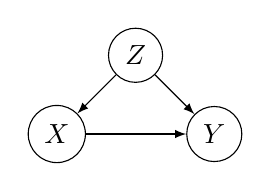
\begin{tikzpicture}
    \path (0,0) node[draw,circle] (X) {$\RV{X}$}
    ++ (1,1) node[draw,circle] (Z) {$\RV{Z}$}
    ++ (1,-1) node[draw, circle] (Y) {$\RV{Y}$};
    \draw[-latex] (X)--(Y);
    \draw[-latex] (Z) -- (Y);
    \draw[-latex] (Z) -- (X);
\end{tikzpicture}
\end{align*}

Then, letting $\model{T}[\RV{XYZ}|\RV{H}]$ be the observational ``see'' model and $\model{T}[\RV{X'Y'Z'}|\RV{HD}]$ be the interventional ``do'' model with $D$ the set of interventions $\{do(\RV{X}=x)\}_{x\in X}$ where we write $x:=do(\RV{X}=x)$ for short, then we know by the backdoor adjustment rule that $\model{T}[\RV{X'Y'Z'}|\RV{HD}]_{hx}^{x'yz} \overset{krn}{=} \model{T}[\RV{Z}|\RV{H}]_h^z \delta[x]^{x'} \model{T}[\RV{Y}|\RV{XZH}]_{hx'z}^y$. 

Let $\model{U}[\RV{ZY}|\RV{XH}] = \model{T}[\RV{Z}|\RV{H}]\rightrightarrows \model{T}[\RV{Y}|\RV{XZH}]$, call $\model{T}[\RV{X}|\RV{H}]$ the ``observational strategy'' and $\model{D}_x[\RV{X}|\RV{D}]_x^{x'} \overset{krn}{=} \delta[x]^{x'}$ the interventional strategies for all $x\in X$. Then we have

\begin{align}
    \model{T}[\RV{XYZ}|\RV{H}] &= \model{U}[\RV{Z}|\RV{H}]\rightrightarrows \model{T}[\RV{X}|\RV{H}] \rightrightarrows \model{U}[\RV{Y}|\RV{XHZ}]\\
    \model{T}[\RV{X'Y'Z'}|\RV{HD}] &\overset{krn}{=} \model{U}[\RV{Z}|\RV{H}]\rightrightarrows \model{D}[\RV{X}|\RV{D}] \rightrightarrows \model{U}[\RV{Y}|\RV{XHZ}]
\end{align}
So this simple example of a Causal Bayesian network is a ``nested comb'' where the outer comb $\model{T}[\RV{XYZX'Y'Z'}|\RV{HD}]$ is the ``see'' and ``do'' models, which are themselves generated by the inner comb $\model{U}[\RV{ZY}|\RV{XH}]$ with different choices $ \model{T}[\RV{X}|\RV{H}]$ and $\model{D}[\RV{X}|\RV{D}]$ for the insert.

This is a simple example, but \citet{jacobs_causal_2019} has used an ``inner comb'' representation of a general class of Causal Bayesian Networks to prove a sufficient identification condition which is itself slightly more general than the identification condition given by \citet{tian2002general}.